\documentclass[tikz,border=2pt]{standalone}
\usepackage{amsmath}
\usepackage{pgfplots}
\pgfplotsset{compat=1.18}
\usetikzlibrary{arrows.meta}
\begin{document}
% Theorem 4.2, Example 1: maximize x1+3x2 over V (corners (2,1),(4,3),(4,14),(-1,4) with values 5,13,46,11);
% walk (2,1) -> (4,3) -> (4,14) along edges to better adjacent corners; at (4,14) the line x1+3x2=46 supports V.
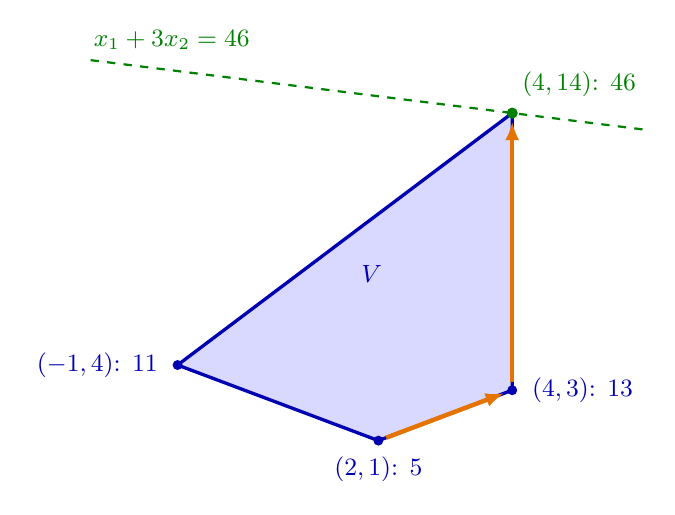
\begin{tikzpicture}[font=\small, >={Latex[length=2.4mm]}, x=0.85cm, y=0.32cm]
  \fill[blue!15] (2,1) -- (4,3) -- (4,14) -- (-1,4) -- cycle;
  \draw[blue!70!black, very thick] (2,1) -- (4,3) -- (4,14) -- (-1,4) -- cycle;
  % supporting level line at the optimum
  \draw[green!50!black, thick, dashed] (-2.3,{(46+2.3)/3}) -- (6,{(46-6)/3});
  \node[green!50!black, anchor=south west, inner sep=1pt] at (-2.3,{(46+2.3)/3+0.3}) {$x_1+3x_2=46$};
  % the walk
  \draw[orange!90!black, line width=1.6pt, ->, shorten <=3pt, shorten >=3pt] (2,1) -- (4,3);
  \draw[orange!90!black, line width=1.6pt, ->, shorten <=3pt, shorten >=3pt] (4,3) -- (4,14);
  % corner points with objective values
  \foreach \p in {(2,1),(4,3),(-1,4)} \fill[blue!70!black] \p circle (1.8pt);
  \fill[green!50!black] (4,14) circle (2pt);
  \node[blue!70!black, anchor=north, inner sep=2pt] at (2,0.6) {$(2,1)$: $5$};
  \node[blue!70!black, anchor=west] at (4.15,3) {$(4,3)$: $13$};
  \node[green!50!black, anchor=south west, inner sep=1pt] at (4.1,14.5) {$(4,14)$: $46$};
  \node[blue!70!black, anchor=east] at (-1.15,4) {$(-1,4)$: $11$};
  \node[blue!70!black] at (1.9,7.6) {$V$};
\end{tikzpicture}
\end{document}
